Social microblogs such as Twitter and Weibo are experiencing explosive growth, with billions of users globally sharing their daily observations and thoughts online. For example, Twitter has more than 255 million average monthly active users (78\% from mobile) since March 31, 2014 and an estimated increase of 25\% per year\footnote{http://solomozone.com/tag/revenues/}. Various studies have shown that Twitter is viable as a social ``sensor'' and holds great promise for detecting and forecasting of significant societal events~\cite{sakaki2010earthquake, bugel2013multilingual}.

In recent years, the phenomenon of bursts and upticks in social media activity has attracted significant attention~\cite{sakaki2010earthquake, lappas2009burstiness, lappas2012spatiotemporal, yin2011geographical, hong2012discovering, eisenstein2010latent, teitler2008newsstand, weng2011event, sayyadi2009event, watanabe2011jasmine, aggarwal2012event}. The relevant methods can be classified into three categories: burst detection, geographical topic modeling, and clustering. Burst detection methods search for space-time regions that have abnormally high counts of some predefined terms~\cite{lappas2009burstiness, lappas2012spatiotemporal}. Sakaki et al. consider spatial-temporal Kalman filtering to track the geographical trajectories of hot spots of Tweets related to earthquakes~\cite{sakaki2010earthquake}. Geographic topic modeling based methods detect topics of interest that are coherent in geographic regions~\cite{yin2011geographical, hong2012discovering, eisenstein2010latent}. Clustering-based approaches search for emerging clusters of documents or terms using predefined similarity metrics that consider factors such as term co-occurrences and social interactions~\cite{teitler2008newsstand, weng2011event, sayyadi2009event, watanabe2011jasmine, aggarwal2012event}.

\begin{figure}[t]
\centering
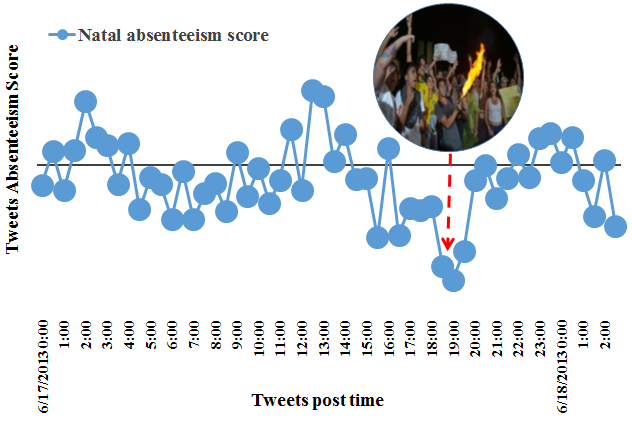
\includegraphics[width=3in]{figures/Natal_example1.png}
\caption{Detected group absenteeism in Natal, Brazil that began at 18:00 hours on June 17, 2013.
This absenteeism event coincides with a large protest that happened in the region.}
\label{fig:natal-protest}
\end{figure}


However, real-world activities are not always correlated with burst signals, and sometimes
are actually associated with unusually low level of activity occurred in social media. As shown in
Figure 1, in the city of
Natal, Brazil, a protest began at 17:00 hrs at the Museum of the Republic, with
people graduatlly joining the demonstration \footnote{http://www.jb.com.br/pais/noticias/2013/06/17/manifestantes-invadem-cobertura-do-congresso-nacional-em-brasilia/}. At the same time, on
Twitter, there was a {\it group absenteeism} behavior from 18:00 to 20:00 hrs on the
same day. As another example, Dec 24, 2013 experienced a
spate of floods in south Brazil. According to the Associated Press, more than 50,000 people have been forced to flee their homes in Minas Gerais and Espirito Santo states. Immediately following the occurrence of
the flood, Twitter activity in this region dropped by 51\%, and reached the lowest point on Dec 24, 2013. Some other examples include bus strikes in Brazil on May 21, 2014, an
earthquake in Chile on Apr 1st, 2014, and power supply disruption in Argentina on Dec 30, 2013
(see Table 2 in Section 4).

Investigating the phenomenon of unusually silent behavior of online users thus
holds enormous potential in understanding local societal events.
This paper presents the first study to systematically investigate the group absenteeism problem, and aims to answer the following three questions:
\begin{itemize}
\item How do we differentiate absenteeism from noise signals?
\item How do we efficiently identify absenteeism groups?
\item How do we gain insight into event detection based on our modeling of group absenteeism?
\end{itemize}

To answer these questions, we first consider the use
of Z-scores to measure the level of standard derivations of a time
series
(e.g., count of Tweets posted)
from its historical average for a given data object
in a given time interval. A lower Z-score is considered as a decreased level of activity. The
measure of absenteeism of a group (subset) of data objects is then defined in terms
of an aggregation function (e.g., summation) of Z-scores of data objects in this group, named as a
group-level Z-score. Secondly, an exhaustive search to identify groups with the lowest group-level Z-score is clearly impractical since there are $2^N$ candidate groups, where $N$ is the total number of data objects. Two different scenarios are considered. In the first scenario, data objects are embedded in a geographic domain and indexed by spatial coordinates. We propose an approach that relaxes convex hulls into rectangles to efficiently identify spatially connected areas as absenteeism groups. In the second scenario, data objects are embedded in a general graph as vertices. We propose an approach that efficiently identifies minimum weighted sub-graphs under sub-graph diameter constraints. To answer the third question, we conduct extensive experiments and discover evidence of significant relationships between the identified absenteeism groups in Twitter and real-world events collected from local news reports (e.g., natural disasters, protests).

\subsection*{Contributions.}
In answering the above research questions, we make several contributions. First, we study the phenomenon of group absenteeism using real Twitter datasets, and discuss useful score functions to measure the degree of absenteeism of a given group of data objects. Second, we formalize the group absenteeism detection problem as a subset minimization problem, and present two efficient approximation algorithms to detect the most absenteeism groups in two different scenarios, respectively: rectangle region search and minimal weight subgraph discovery. Finally, we conduct extensive experiments to analyze the strengths and weakness of these two algorithms and demonstrate their application to studying Twitter datasets over Latin America.

\iffalse
The rest of the paper is organized as follows. Section~\ref{sec:related} reviews related work and existing methodologies. Section~\ref{sec:algorithm} formalizes the group absenteeism problem, presents useful score functions, and designs efficient approximation algorithms. Section~\ref{sec:experiemnt} presents extensive experiments and comparisons, and Section ~\ref{sec:conclusion} suggests directions for future work.
\fi


%\begin{figure}[t]
%	\centering
%	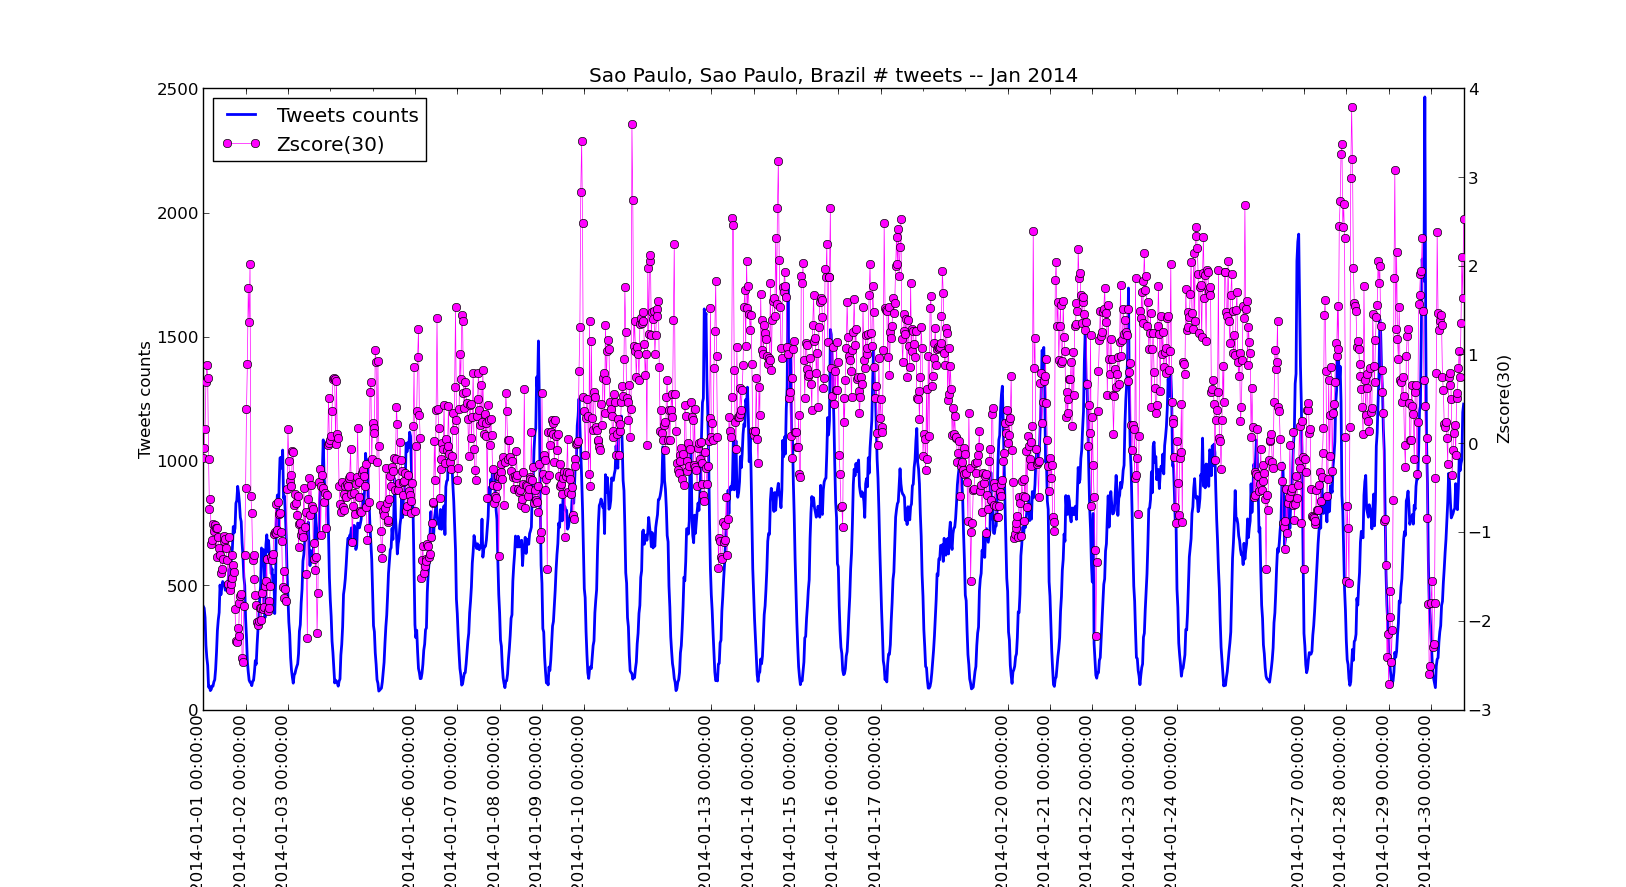
\includegraphics[width=3.3in, height=1.6in]{figures/tweets-period.png}
%	\caption{Tweets volume of January 2014 of Sao Paulo, Brazil. Blue curve shows tweets volume, and purple curve shows tweets zscore.
%	}
%	\label{fig:Tweets_volume}
%\end{figure}
%
%
%From Figure~\ref{fig:Tweets_volume}, we can see the Twitter activity has obvious periodicity of rises and falls pattern. Generally speaking, weekday has higher volume than weekends, and after midnight tweets tends inactive until the next day working time. To differentiate absenteeism signals from noise signals, we consider Z-score to measure for one time interval, how many standard derivations from its historical average for a given data object (e.g., count of tweets posted in a specific city).
%A $Z-score$ is defined by:
%\begin{equation}
%	\label{eq:zscore}
%	\begin{array}{l}
%		Z-score_t(n) =(X-\mathcal{M})/{\Sigma}\,
%	\end{array}
%\end{equation}
%where $X$ is the Twitter volume at time interval $t$, $\mathcal{M}$ is the trailing $n$-day moving average of the Twitter volume at time $t$, and $\Sigma$ is the standard deviation of those trailing $n$-day moving Twitter volume at time $t$. A lower Z-score is considered as the decreased level of activity of this data object. The measure of absenteeism of a group (subset) of data objects is defined as an aggregation function (e.g., summation) of Z-scores of data objects in this group, named as group-level Z-score. The detection of group absenteeism can be formulated as the identification of groups that have minimum group-level Z-score.
%
